\documentclass{../notatki}

\title{Wstęp do Fizyki Kwantowej}

\begin{document}

\section{Wstęp}

\subsection{Fizyka Klasyczna}

Zwyczajowo, określa się, że fizyka klasyczna jest całym korpusem fizyki,
opracowanym przed pojawieniem się fizyki kwantowej. Historycznie zatem,
jest to fizyka opracowana przed XX wiekiem, opracowana przez Newtona, Leibniza,
Maxwella, et. al.

\begin{itemize}
  \item Mechanika - Newton + Leibniz + Lagrange + Hamilton
  \item Elektrodynamika - Maxwell
  \item Termodynamika
  \item Fizyka statystyczna
\end{itemize}

\subsubsection{Mechanika}

Cała mechanika opiera sie na trzech prawach Newtona:
\begin{enumerate}
  \item $
    \vec{F} = m\vec{a}
    $
  \item $
    \frac{\vec{dp}}{dt} = \vec{F}
    $
  \item Każda akcja ma przeciwną i równą reakcję.
\end{enumerate}

Z tych praw wynika cała mechanika, wraz z alternatywnymi ujęciami, takimi jak
równania Lagrange'a i Hamiltona.

\subsubsection{Elektrodynamika}

Cała elektrodynamika wywodzi się z równań Maxwella:
\begin{enumerate}
  \item $\nabla \vec{E} = \frac{q}{\epsilon_0}$
  \item $\nabla \vec{B} = 0$
  \item $\nabla \times \vec{E} = -\frac{\partial \vec{B}}{\partial t}$
  \item $\nabla \times \vec{B} = \mu_0 \vec{J} + \mu_0 \epsilon_0
    \frac{\partial \vec{E}}{\partial t}$
\end{enumerate}

\subsection{Widmo absorpcji}

W momencie, gdy światło przechodzi przez gazową postać pierwiastka, a następnie
pryzmat, światło zamiast rozszczepić się na wszystkie kolory, rozszczepia się
na prawie wszystkie kolorym, pozostawiając luki w spektrum. To zjawisko
nazywane jest widmem absorpcji.

Wynika ono z zachowania elektronów w atomach pierwiastka, które po trafieniu
przez foton, zmieniają swój stan energii, co powoduje zmianę długości fali
światła i co za tym idzie luki w spektrum.

$$
\frac{1}{\lambda} = R \left( \frac{1}{n_1^2} - \frac{1}{n_2^2} \right)
$$

To zjawisko dowodzi tego, że poziomy energetyczne elektronów są skwantyzowane,
czyli dyskretne. Na podstawie tego zjawiska opracowano model atomu Bohra, w
którym atomy znajdują się na dyskretnych orbitalach dookoła jądra atomu.
Przejście między tymi stanami energii kosztuje energię.

Dla atomu i elektronu na orbitalu w odległości $r$ od jądra atomu:
$$
m \frac{v^2}{r} = \frac{1}{4 \pi \epsilon_0} \frac{e^2}{r^2}
$$
$$
mvr = n\hbar \rightarrow \text{promieniowanie jest absorbowane}
$$
$$
\text{promieniowanie} \leftrightarrow \text{zmiana orbity}
$$

\subsection{Katastrofa w ultrafiolecie}

Poszukiwania zdolności emisyjnej ciał, doprowadziły do powstania
prawa Rayleigha-Jeansa:
$$
f(\nu, T) = 2 \frac{\nu^2}{c^2} kT
$$
$$
f(\lambda, T) = 2 \frac{ckT}{\lambda^4}
$$
Zcałkowanie tego prawa, po całym zakresie częstości, daje nam nieskończenie dużą
energię. To jest niemożliwe. Co więcej, w komorze, będącej ciałem
doskonale czarnym, promieniowanie ultrafioletowe zgodnie z tym prawem
powinno w nieskończoność wydzielać energię. To oczywiście nie było
zgodne z obserwacjami. Tą sprzeczność nazwano katastrofą w ultrafiolecie.

\subsection{Energia relatywistyczna}

Energia cząsteczki w ruchu to:
$$
E^2 = p^2c^2 + m^2c^4
$$

\section{Efekt Fotoelektryczny}

W wyniku promieniowania fotonami, elektrony atomów pierwiastka są
wyrzucane z atomu. Efekt ten jest wykorzystywany w praktyce w
napędzaniu fotodiod i fotokomórek.

Energia fotonu zależy od charakterystyk fali, w tym długości fali $\lambda$:
$$
E_f = h\nu = \hbar \omega = \frac{hc}{\lambda} = pc
$$
Foton padając na materiał powoduje wyrzucenie elektronu naładowanego
$U$ z energią kinetyczną $E_{k \text{max}}$. W wyniku tego procesu
utracona zostaje energia w postaci pracy wyjścia $W$:
$$
E_{k \text{max}} = E_f - W = eU
$$
Częstością progową nazywamy najniższą częstość $\omega_0$, dla której
$E_{k \text{max}} = 0$.

\section{Zjawisko Comptona}

W zjawisku Comptona foton padający na elektron zmienia kierunek i
częstość. Efekt ten jest wykorzystywany w praktyce w analizie struktury
atomów i molekuł.

\begin{figure}[h]
  \centering
  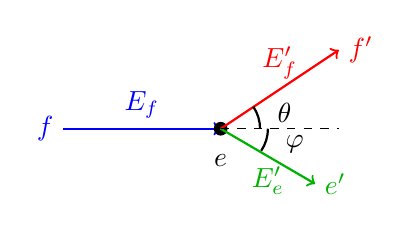
\begin{tikzpicture}
    \draw[->,thick,blue] (-2,0) -- (0,0) node[midway,above] {$E_f$};
    \draw[blue] (-2,0) node[left] {$f$};

    \draw[fill=black] (0,0) circle (0.08);
    \draw (0,-0.2) node[below] {$e$};

    \draw[->,thick,red] (0,0) -- (1.5,1) node[midway,above] {$E_f'$};
    \draw[red] (1.5,1) node[right] {$f'$};

    \draw[->,thick,green!70!black] (0,0) -- (1.2,-0.7)
    node[midway,below] {$E_e'$};
    \draw[green!70!black] (1.2,-0.7) node[right] {$e'$};

    \draw[thick] (0.5,0) arc (0:34:0.5);
    \draw (0.6,0.2) node[right] {$\theta$};

    \draw[thick] (0.6,0) arc (0:-34:0.5);
    \draw (0.7,-0.2) node[right] {$\varphi$};

    \draw[dashed] (0,0) -- (1.5,0);
  \end{tikzpicture}
  \caption{Ilustracja zjawiska Comptona. Foton $f$ ma długość fali $\lambda$.}
\end{figure}

W zjawisku zachowanny jest pęd oraz energia, co wraz z równaniem Comptona:
$$
(\lambda' - \lambda) \frac{m_ec}{h} = 1 - \cos\theta
$$
Pozwala nam w istocie wyprowadzić wszystkie niewadome w zjawisku.

$$
p_f + p_e = p_f' + p_e' \Rightarrow
\begin{cases}
  \frac{h}{\lambda} = \frac{h}{\lambda'}\cos\theta + p_e\cos\varphi \\
  0 = \frac{h}{\lambda'}\sin\theta + p_e\sin\varphi
\end{cases}
$$

$$
E_f + E_e = E_f' + E_e' \Rightarrow \frac{hc}{\lambda} + m_ec^2 =
\frac{hc}{\lambda'} + E_e'
$$

\end{document}
